\section{ガイダンス}
%
%%% GOAL
%
\subsection{科目の概要}
\begin{frame}
\frametitle{科目の概要}
  \begin{itemize}
\item 学期: 水曜日 3-4 限
\item 場所: 南 4 号館 3 階第 2 演習室
\item 担当教員: 永藤 直行 (ナガトウ ナオユキ)
\item 問い合わせ先: nagatou@presystems.xyz
\item 質問はメイルで,対面(石川台 8 号館 317)は水曜日 15:00- 以降
\item 永藤担当クラスのサイト: \href{https://sites.google.com/presystems.xyz/elementarycs/top}{\beamerbutton{https://sites.google.com/presystems.xyz/elementarycs/top}} 
\item 共通サイト: \href{https://wakita.github.io/classes/years/y23/cs1/course.html}{\beamerbutton{https://wakita.github.io/classes/years/y23/cs1/course.html}}
\item 板書: \href{https://mitou-my.sharepoint.com/:o:/g/personal/nnagato_mitou_org/Ei5nV0iuNsRJlWDG4f5NAHkBINXV2nMagLjcqF1uL2BfJA?e=bbc0sd}{\beamerbutton{Onenote}} に置いておきます
\item その他ツールや参考図書は必要に応じて URL を示します
  \end{itemize}
\end{frame}
%\begin{frame}
%\frametitle{TA の方々}
%  \begin{itemize}
%\item TA の方の自己紹介
%\item \href{https://drive.google.com/file/d/1-2OaOLna8_Uu9AtbSWEXsvDjGBzugo0e/view}{\beamerbutton{DSAI}}のご案内
%  \end{itemize}
%\end{frame}
%
%%% REFERENCE
%
\subsection{参考図書}
\begin{frame}
\frametitle{参考図書}
  \begin{itemize}
\item 渡辺治 著,コンピュータサイエンス\textendash 計算を通して世界を観る, 丸善出版 (2015)
\item Kenneth H. Rosen 著, Discrete Mathematics and Its Applications 8th ed.(2018)
  \end{itemize}
  \begin{columns}[t]
    \begin{column}{0.45\textwidth}
\centering

\includegraphics[scale=.25]{./Figure/TextBook.jpg}
    \end{column}
    \begin{column}{0.45\textwidth}
\centering
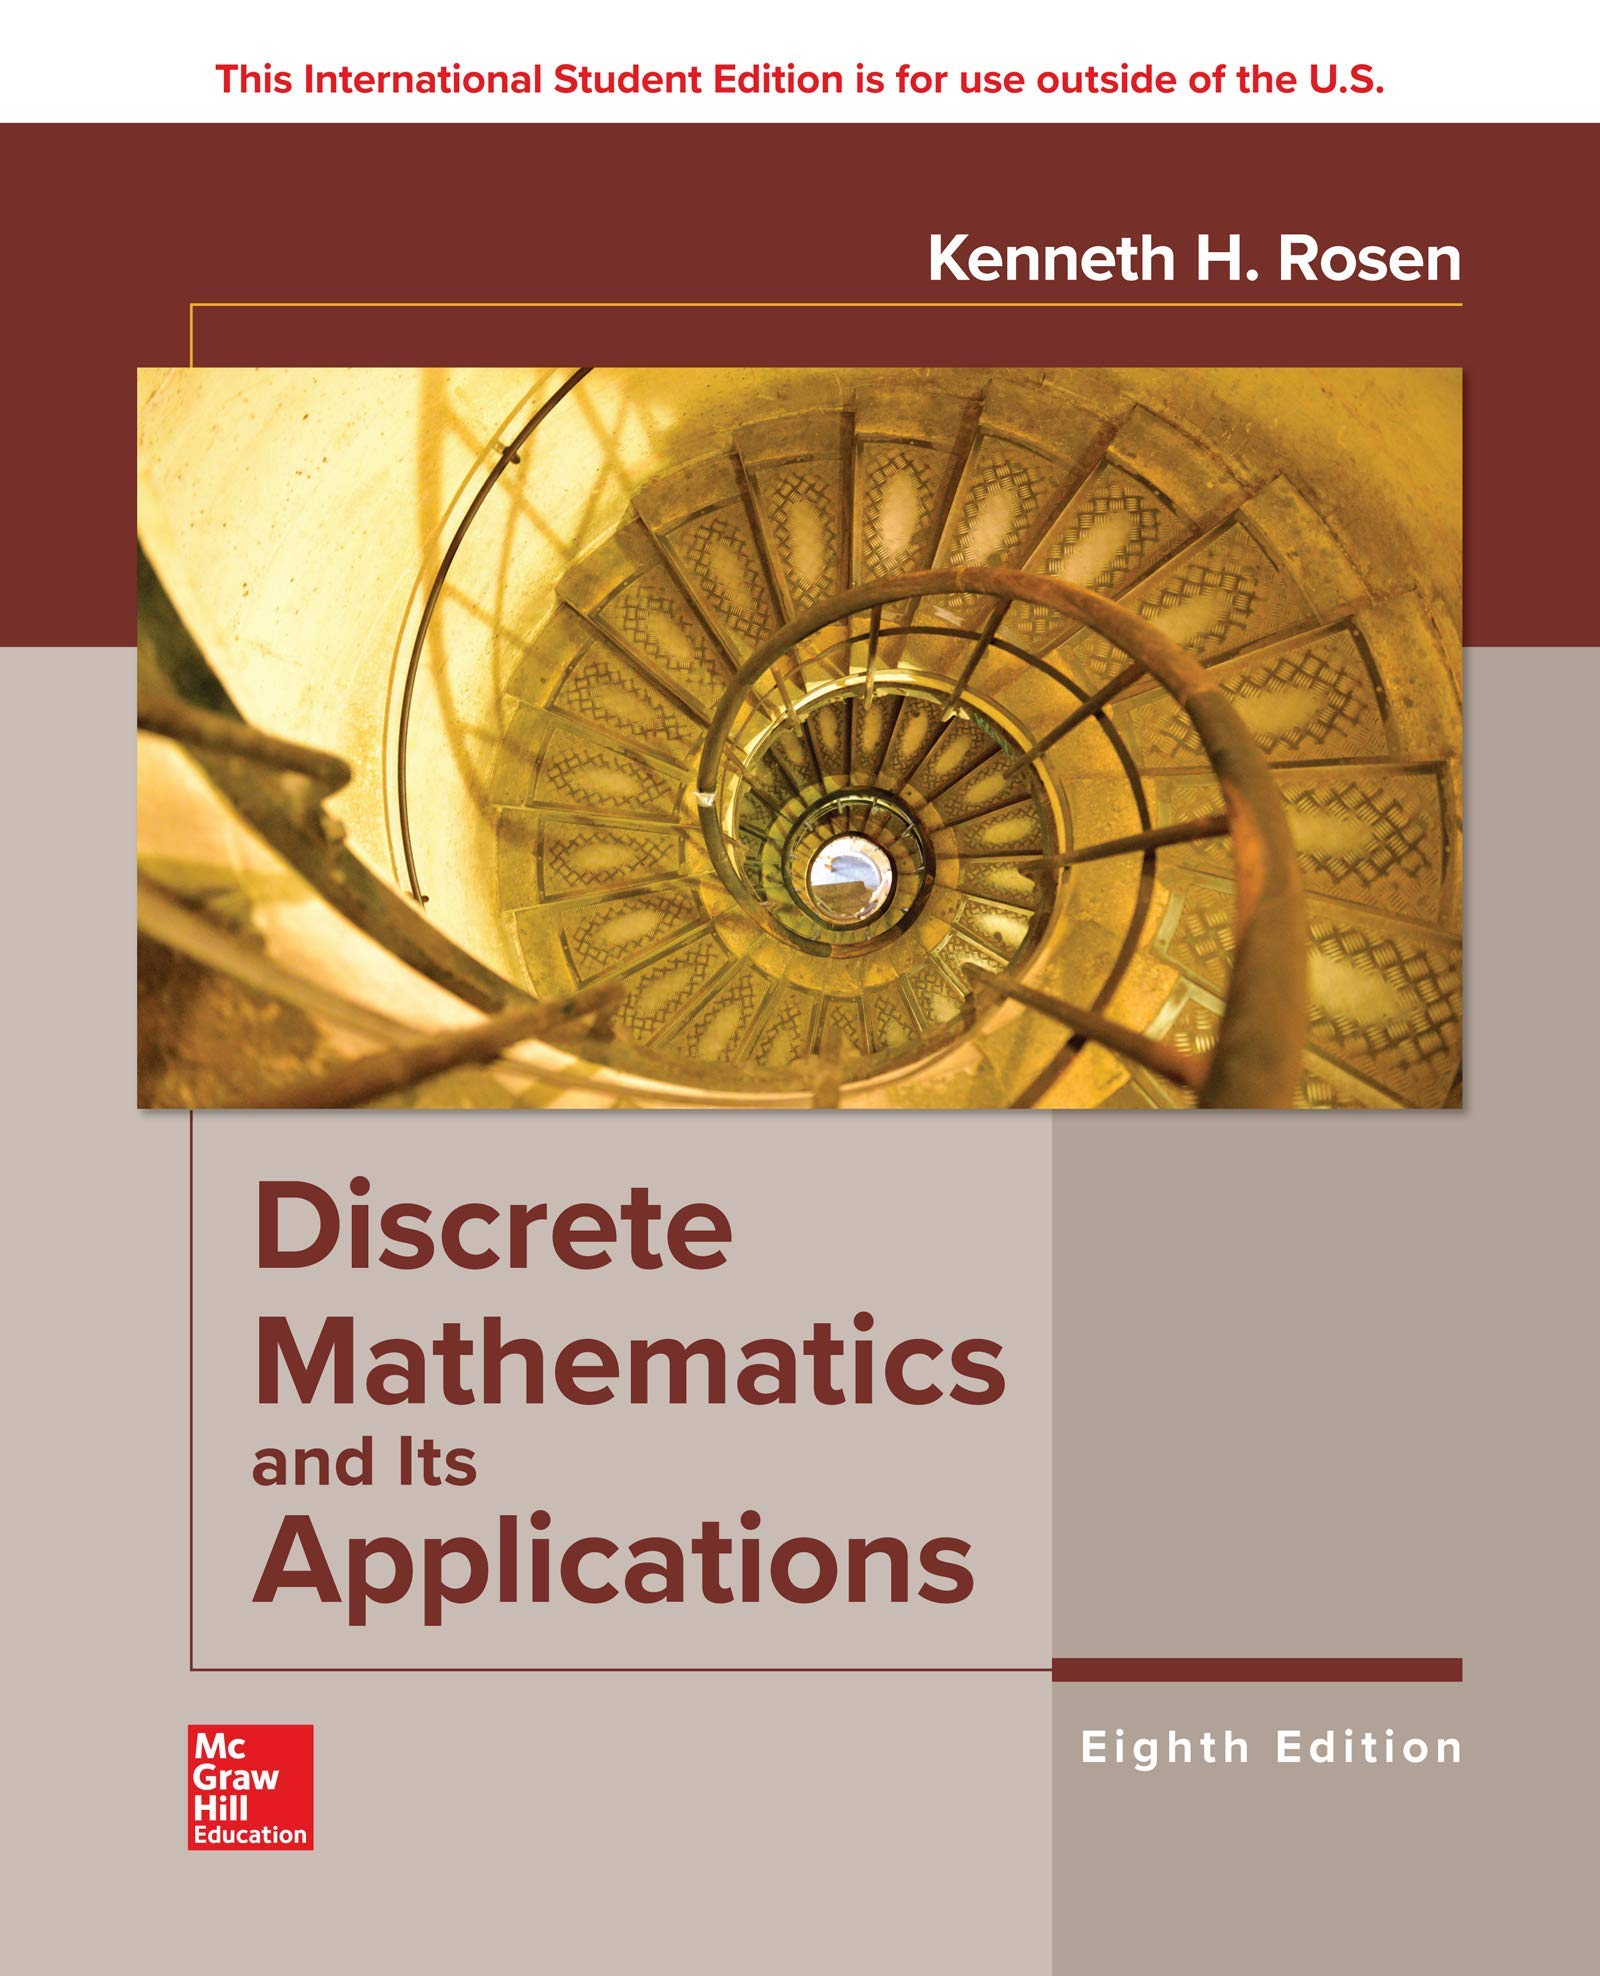
\includegraphics[scale=.07]{./Figure/DMA.jpg}
    \end{column}
  \end{columns}
\end{frame}
%
%%% EVALUATION
%
\subsection{評価基準}
\begin{frame}
\frametitle{評価基準}
  \begin{itemize}
\item 講義は全 7 回,期末試験は行いません
\item 宿題: 3 回 全部で \(10\) 点
\item 課題: 3 回 \(25+25+25=75\) 点
\item 特別課題: 1 回 \(15\) 点(提出任意)
\item 課題提出: 
    \begin{itemize}
\item 宿題,課題の提出方法はその都度指定します
    \end{itemize}
  \end{itemize}
\end{frame}
%
%%% 3rd Quarter Schedule
%
%\subsection{講義内容}
%\begin{frame}
%\frametitle{講義内容}
%  \begin{enumerate}
%\item 計算の基礎
%\item 配列,文字列
%\item 暗号入門
%  \end{enumerate}
%\end{frame}
